\documentclass[a4paper]{article}

\usepackage[english]{babel}
\usepackage[utf8]{inputenc}
\usepackage{graphicx}
\usepackage{enumitem}
\graphicspath{ {./images/} }
    
\title{CS2200 Homework 2}
\author{Evan Wilcox}
\setlength\parindent{0pt}
    
\date{Due Feburary 14, 2019}
    
\begin{document}
    \maketitle

    \begin{enumerate}

    \item 
    The two functions give the same result because $f(n)$ increments $n$ until $n-10$
    is greater than 100 then prints $n$, while $g(n)$ justs prints 91 or $n-10$ which 
    ever is greater.\\
    
    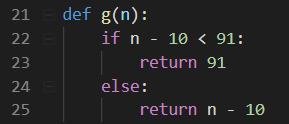
\includegraphics[scale=0.6]{1a} \\
    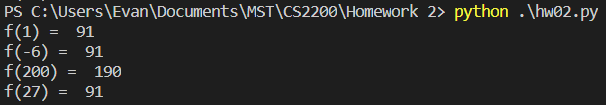
\includegraphics[scale=0.6]{1b}

    \item 
    A(3, 4) was the maximum value my computer was able to computer, for any greater
    values the Maximum Recursion Depth reached was given. \\ 
    A(2, 2) produces the following chain of calls: 
    
    A(2, 2), A(2, 1), A(2, 0), A(1, 1), A(1, 0), A(0, 1), A(0, 2), A(1, 3), \\ A(1, 2), 
    A(1, 1), A(1, 0), A(0, 1), A(0, 2), A(0, 3), A(0, 4), A(1, 5), \\ A(1, 4), A(1, 3),
    A(1, 2), A(1, 1), A(1, 0), A(0, 1), A(0, 2), A(0, 3), \\ A(0, 4), A(0, 5), A(0, 6).
    
    For a total of 27 calls.
    
    \newpage
    \item 
    Prove by induction that for any natural number $n$
    $$\frac{1^{2}}{1\cdot3} + \frac{2^{2}}{3\cdot5} + \frac{3^{2}}{5\cdot7} + ... + \frac{n^{2}}{(2n-1)(2n+1)} = \frac{n(n+1)}{2(2n+1)}$$


    \textbf{Define the problem.} \\
    If $$f(n) = \frac{1^{2}}{1\cdot3} + \frac{2^{2}}{3\cdot5} + \frac{3^{2}}{5\cdot7} + ... + \frac{n^{2}}{(2n-1)(2n+1)}$$
    and $$g(n) = \frac{n(n+1)}{2(2n+1)}$$

    then $P(n)$ is true when $f(n) = g(n)$. Prove $P(n)$ is true for all 
    natural numbers. \\
    
    \textbf{Stopping value and two more.}

    $f(1) = \frac{1^{2}}{1\cdot3} = \frac{1}{3}$ \\
    $g(1) = \frac{1(1+1)}{2(2+1)} = \frac{1}{3}$ \\
    $f(2) = \frac{1^{2}}{1\cdot3} + \frac{2^{2}}{3\cdot5} = \frac{1}{3} + \frac{4}{15} = \frac{3}{5}$\\
    $g(2) = \frac{2(2+1)}{2(2\cdot2+1)} = \frac{3}{5}$ \\
    $f(3) = \frac{1^{2}}{1\cdot3} + \frac{2^{2}}{3\cdot5} + \frac{3^{2}}{5\cdot7} = \frac{1}{3} + \frac{4}{15} + \frac{9}{35}= \frac{6}{7}$\\
    $g(3) = \frac{3(3+1)}{2(2\cdot3+1)} = \frac{6}{7}$ \\

    \textbf{Inductive Case.} \\
    $f(n) = f(n-1) + \frac{n^{2}}{(2n-1)(2n+1)}$ \\ 
    $= g(n-1) + \frac{n^{2}}{(2n-1)(2n+1)}$ \\
    $= \frac{(n-1)(n)}{2(2(n-1)+1)} + \frac{n^{2}}{(2n-1)(2n+1)}$ \\
    $= \frac{n^{2}-n}{2(2n-1)} + \frac{n^{2}}{(2n-1)(2n+1)}$ \\
    $= \frac{n^{2}-n}{2(2n-1)} \cdot \frac{2n+1}{2n+1} + \frac{n^{2}}{(2n-1)(2n+1)} \cdot \frac{2}{2}$ \\
    $= \frac{(n^{2}-n)(2n+1)}{2(2n-1)(2n+1)} + \frac{2n^{2}}{2(2n-1)(2n+1)}$ \\
    $= \frac{(n^{2}-n)(2n+1)+2n^{2}}{2(2n-1)(2n+1)}$ \\
    $= \frac{n(2n^{2}+n-1)}{2(2n-1)(2n+1)}$ \\
    $= \frac{n(2n-1)(n+1)}{2(2n-1)(2n+1)}$ \\
    $= \frac{n(n+1)}{2(2n+1)}$ \\
    $= g(n)$ \\

    \textbf{Conclusion.} \\
    Because $P(n)$ is true for for all $n$ we can conclude that 
    $$\frac{1^{2}}{1\cdot3} + \frac{2^{2}}{3\cdot5} + \frac{3^{2}}{5\cdot7} + ... + \frac{n^{2}}{(2n-1)(2n+1)} = \frac{n(n+1)}{2(2n+1)}$$




    \newpage
    \item Prove by induction that the sum of the cubes of 3 consecutive natural 
    numbers is divisible by 9. \\

    \textbf{Define the problem.} \\
    The property $P(n)$ is true when 
    $$(n)^{3}+(n+1)^{3}+(n+2)^{3} \; \% \; 9 == 0$$
    Prove that $P(n)$ is true for all natural numbers $n$. \\

    \textbf{Stopping value and two more.} \\
    $(1)^{3}+(1+1)^{3}+(1+2)^{3} = 1+8+27 = 36\; \% \; 9 == 0$ \\
    $(2)^{3}+(2+1)^{3}+(2+2)^{3} = 8+27+64 = 99\; \% \; 9 == 0$ \\
    $(3)^{3}+(3+1)^{3}+(3+2)^{3} = 27+64+125 = 216\; \% \; 9 == 0$ \\

    \textbf{Inductive Case.} \\ 
    Try $n+1$. 

    $(n+1)^{3}+(n+2)^{3}+(n+3)^{3} \; \% \; 9 == 0$ \\
    $(n+1)^{3}+(n+2)^{3}+(n+3)(n^{2}+6n+9) \; \% \; 9 == 0$ \\
    $(n+1)^{3}+(n+2)^{3}+n^{3}+9n^{2}+27n+27 \; \% \; 9 == 0$ \\
    $9n^{2}+27n+27 \; \% \; 9 == 0$ 
    
    Because we assume $(n)^{3}+(n+1)^{3}+(n+2)^{3}$ is divisible by 9 and all other
    terms are also divisible by 9 we can say $P(n)$ is true for all $n$. \\
 
    \textbf{Conclusion.} \\
    Because $P(n)$ is true for all $n$ we can conclude that the sum of the cubes of 
    3 consecutive natural numbers is divisible by 9.





    \newpage
    \item Prove by induction that the version of insertion sort given in Lecture
    4 is correct. In other words, prove that if you input a list of integers, you will
    output a sorted list of integers. \\

    \textbf{Define the problem.} \\
    Prove that Insertion sort sorts for any given array of integers. \\

    \textbf{Base Case.} \\
    The base case of insertion sort is an array of length zero, an empty array and this array
    is always sorted. \\

    \textbf{Inductive Case.} \\
    When insertion sort inserts a new element to the array, it inserts it in to a sorted
    array. So the array stays sorted until all elements are inserted. \\

    \textbf{Conclusion.} \\
    After showing the last two steps, we can conclude that insertion will sort an array
    of integers.



    \end{enumerate}

\end{document}